\makeatletter
\def\@makechapterhead#1{%
  \vspace*{10\p@}%
  {\parindent \z@ \raggedleft \normalfont
    \ifnum \c@secnumdepth >\m@ne
      \if@mainmatter
        \LARGE\bfseries \@chapapp\space \thechapter
	\vskip 4pt
        \hrule height 2pt
        \par\nobreak
        \vskip 5\p@
      \fi
    \fi
    \interlinepenalty\@M
    \huge \bfseries #1\par\nobreak
\vskip 5pt

\hrule height 2pt   
 \vskip 10\p@  
  }}
\makeatother

\chapter{Microcontrollers}\label{chap7}
\addtocontents{toc}{\protect\contentsline{chapter}{\protect Chapter \numberline{\thechapter.}
Microcontrollers}{\thepage--\pageref{7end}}}  

\section{Introduction to Microcontrollers}\label{sec7.1}

Till now, we have learnt that there are different types of digital logic elements like AND gate, NAND gate, NOR gate etc. and several logic circuits like Adders, Flip-flops etc. can be implemented using basic gates. All these circuits are implemented physically in the form of an {\em Integrated circuit} (IC) or commonly known as ``Chip'' and are given part numbers to identify. For example, IC 7400 is a Quad 2-input NAND gate (i.e., it contains four 2-input NAND gates), IC 7483 is a 4-bit binary parallel Adder and so on. Note that each IC performs only one logic function.

However, when we need to design a logic system we need to use multiple such ICs. This would result in a very complex hardware with increase in cost as well. In order to reduce the hardware and cost, companies like Intel, Motorola, AMD, Atmel etc. started developing ICs (that contains multiple logic circuits inside) which can be used for real-life applications. This lead to the ``digital revolution'' what we are seeing today in the area of consumer electronics, office automation, automobiles etc.

\medskip
\heading{Microcontrollers}
\begin{itemize}
\item A microcontroller is a ``Programmable digital logic device'' fabricated on a single VLSI (Very Large Scale Integration) chip that contains a processor core, and other logic blocks like RAM, ROM, Timer, IP/O/P parts etc. on the chip itself.

\item A microcontroller (also known as embedded processor) is basically used to perform only few specific tasks unlike CPU (Microprocessor) of a computer which is used for general purpose computational activities. 

\item Microcontrollers were initially developed during 1980s by companies like Intel, Motorola, AMD, etc.

\item Major goals in developing Microcontrollers are: decreasing power consumption, reducing cost of the system and reducing the physical size of the system (if making system {\em portable}).
\end{itemize}

\medskip
\heading{Applications of Microcontrollers}
\medskip

Most of the Embedded systems and Gadgets we are using today have Microcontrollers $(\mu \text{C}_{\text{s}})$ as programming and controlling device. For example, in consumer Electronics domain $(\mu \text{C}_{\text{s}})$ are used in Fax machines, Musical instruments, Washing Machines, Ovens, Painters, Security Systems, Remote Controls, Mobile Phones, HDTVs, Camcorders, Digital Cameras, Video gaming devices, Toys and so on. Similarly, considering Automobiles $\mu \text{C}_{\text{s}}$ are used for ABS, EBD, Transmission control, Entertainment etc. We can see that $\mu \text{C}_{\text{s}}$ are being used in almost every digital product. We are using in today's world.

\medskip
\heading{Intel 8051 Microcontroller}
\begin{itemize}
\item Intel Inc. developed the first 8-bit Microcontroller 8051 in the year 1981. This $\mu \text{C}$ has 128 bytes of RAM, 4k bytes of ROM, two 16-bit Timers, one serical part, four 8-bit parallel parts along with a CPU core on a single chip.
\end{itemize}

\noindent
{\bf Note~:} RAM (Random Access Memory which is volatile) 

ROM (Read-Only Memory which is non-volatile)
\begin{itemize}
\item Many other versions of basic 8051 like 8031, 8052, 8032, 8751, 8951 were developed from Intel and Atmel.

\item Fig.~\ref{fig7.1} shows the 8051 architectures block diagram.

\item Lets briefly discuss the architectural blocks shown in Fig.~\ref{fig7.1}.
\begin{itemize}
\item 8051 is a 8-bit Microcontroller i.e., the CPU can work with only 8-bit data at a time.

\item 8051 works with a clock frequency of 11.0592 MHz using an on-chip oscillator.

\item 8051 has internal RAM (data memory) of 128 byes. This is organized into 4 Register banks, Scratch pad and bit addressable memory area. Each register bank contains eight 8-bit resisters named as RO to RT.

\item 8051 contains 4k bytes of on-chip ROM (program memory).

\item There are two 16-bit Timers/counters which can be used for timing applications.
\begin{figure}[H]
\centering
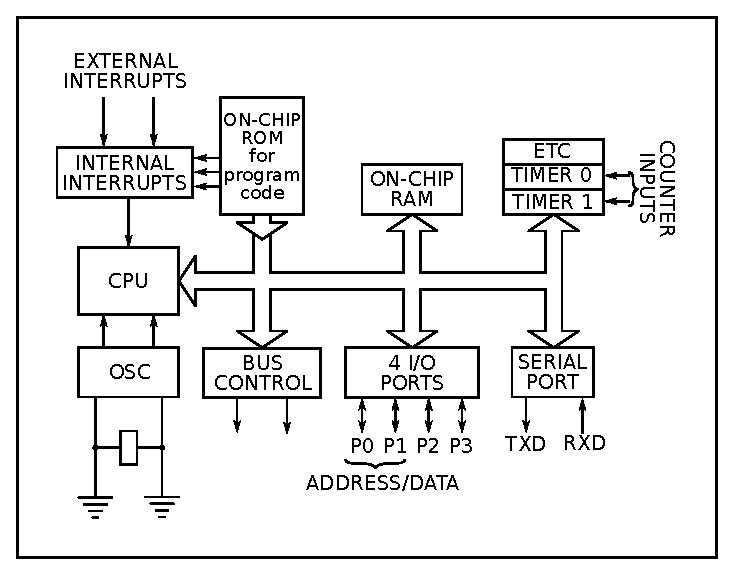
\includegraphics[scale=.95]{chap7/fig7.1.eps}
\caption{Inside the 8051 Microcontroller Block Digram}\label{fig7.1}
\end{figure}

\item The interrupt control logic is designed to handle external and internal interrupts (external registers and internal exception conditions).

\item 8051 has four 8-bit input output (I/O) parallel ports named as P0, P1, P2, P3. Each part is bidirectional and can be used to connect external device like ADC, DAC, Motors, Printers, LEDs, LCDs, 7-segment display etc. to the 8051. The parts can be used for data transfer between $\mu$C and external device.

\item 8051 also has a {\em serial-part} that can be used for serial communication. For example, this can be used to connect 8051 IC to a desktop computer using RS-232 part of Computer.
\end{itemize}
\end{itemize}

\heading{8051 Pin Configuration}
\begin{itemize}
\item Fig.~\ref{fig7.2} shows the Pin diagram of 8051. The pins are used to connect (interface) external devices with $\mu$C.
\begin{figure}[H]
\centering
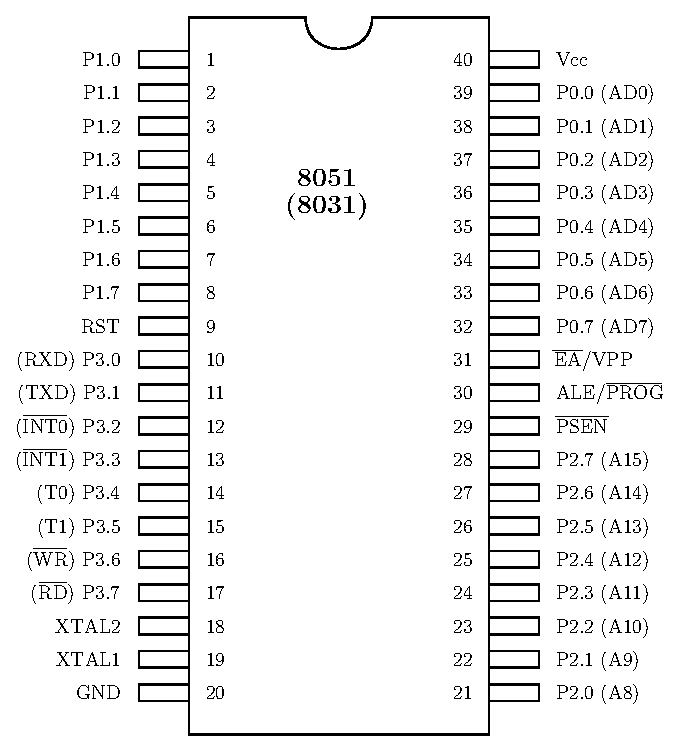
\includegraphics[scale=.85]{chap7/fig7.2.eps}
\caption{8051 Pin Diagram}\label{fig7.2}
\end{figure}
\end{itemize}

\heading{Stepper Motor Interfacing}
\begin{itemize}
\item A `Stepper Motor' is a device that translator electrical pulses to mechanical movement. Stepper motors are used in a dot matrix printers, analog clocks, robotics and so on for position control.

\item The most common stepper motors have four stat or windings (A, B, C, D) with a center tapped common as shown.
\begin{figure}[H]
\centering
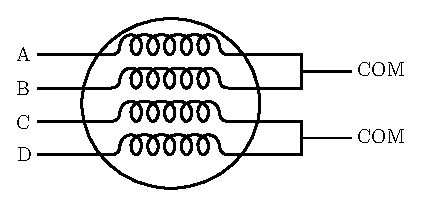
\includegraphics{chap7/fig7.3.eps}
\end{figure}

\item The stepper motor shaft moves in a fixed repeatable increment called `step angle' (usually 1.8$^{\circ}$).

\item The direction of the rotation is controlled by stator poles, when current pulses are sent to the windings (say in A, B, C, D orders) motor rotates in one direction. As the direction of current is changed, the polarity is also changed causing reversal of the direction.

Fig.~\ref{fig7.3} shows the connection of Stopper motor to 8051.
\begin{figure}[H]
\centering
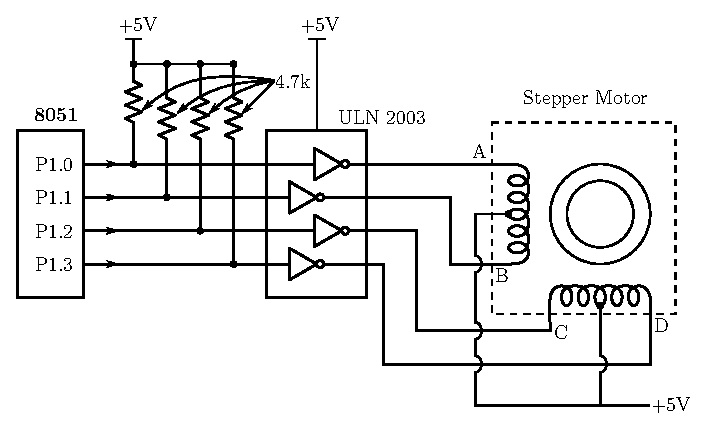
\includegraphics{chap7/fig7.4.eps}
\caption{Interfacing stopper motor to 8051}\label{fig7.3}
\end{figure}

\item The four stater winding are controlled by four part pins (P1.O-P1.3) of Part 1. Line drivers like ULN 2003 is used to enhance current supplied to the windings.

\item When current pulse is given to energize a winding (say A) coil, motor moves by one step (say $1.8^{\circ}$). $\therefore$ we need 4-step switching sequence to switch ON the windings. To complete one revolution. motor has to make 200 steps $(200\times 1.8=360^{\circ})$. So, we need 50 cycles of 4-step sequence to energize the windings.

\item As indicated earlier, 8051 is a ``Programmable'' device i.e., user can give instructions (called mnemonics) to 8051 to perform arithmetic or logic operations. Data can be transferred through Part 1 to energetic motor winding there instructions. 
\end{itemize}


\label{7end}
